\documentclass[a4paper,twocolumn]{article}
\usepackage[a4paper,margin=2cm]{geometry} % Seitenränder anpassen
\usepackage{graphicx} % Für Grafiken
\usepackage{amsmath, amssymb} % Für mathematische Formeln
\usepackage{hyperref} % Für Hyperlinks
\usepackage{caption} % Für Bildunterschriften
\usepackage[printonlyused]{acronym}
\usepackage{pgffor} % Paket für die foreach-Schleife
\usepackage{shellesc} % Für das Ausführen von Shell-Befehlen (mit pdflatex -shell-escape)
\usepackage{todonotes}

% Abstand zwischen den Spalten erhöhen
\setlength{\columnsep}{1cm} 

\title{Augmented Reality with Aruco Markers}
\author{
    Hochschule Ravensburg-Weingarten \\[1em] % Hochschule zentriert
    \begin{minipage}[t]{0.45\textwidth} % Linke Spalte
        \centering
        Jonas Alber \\ % Name
        \texttt{jonas.alber@hs-weingarten.de} % E-Mail
    \end{minipage}
    \hfill
    \begin{minipage}[t]{0.45\textwidth} % Rechte Spalte
        \centering
        Tim Schweitzer \\ % Name
        \texttt{tim.schweitzer@hs-weingarten.de} % E-Mail
    \end{minipage}
}
\date{\today}

\begin{document}

\maketitle

\section*{Disclaimer}

Der Inhalt dieses Dokuments wurde von den oben genannten Autoren erstellt. Zur Verbesserung der Lesbarkeit wurde ChatGPT von OpenAI genutzt. Sämtliche Inhalte wurden jedoch von den Autoren geprüft und gegebenenfalls angepasst.


\section*{Abkürzungsverzeichnis}
\begin{acronym}[RWU]
    \acro{RWU}{Hochschule Ravensburg Weingarten}
    \acro{AI}{Artificial Intelligence}
    \acro{IoT}{Internet of Things}
\end{acronym}

\begin{abstract}

\end{abstract}

\section{Einleitung}

\subsection{Aufgabenstellung}
Diese Arbeit wurde im Rahmen des Fachs Computer Vision an der \ac{RWU} als Projektaufgabe erstellt. Ziel des Projekts ist es, mithilfe der Bibliothek OpenCV Bilder so zu modifizieren, dass ein Poster derart in das Bild integriert wird, dass für den Betrachter der Eindruck entsteht, das Poster befinde sich tatsächlich im Raum.
\\
Diese Bildaugmentierung wird auf einen vorgegebenen Datensatz angewendet, wobei die erzielten Ergebnisse anschließend auf selbst erstellte Bilder übertragen werden sollen.

\subsection{Marker}
\todo{Fehlende Quelle!}
Eine zentrale Herausforderung in allen Disziplinen der Informatik, die mit Bilddaten arbeiten, besteht in der Interpretation von Räumlichkeiten auf Basis einzelner Perspektiven. Ein vielversprechender Ansatz zur Erkennung von Orientierung und Ausrichtung ist die Nutzung von Markern.
\\
Im Rahmen dieser Arbeit wird der ArUco-Marker eingesetzt. Dabei handelt es sich um speziell entwickelte Marker, die aus einem quadratischen schwarz-weißen Muster bestehen und eine eindeutige Identifizierung sowie die Berechnung von Position und Ausrichtung im Raum ermöglichen.
\subsection{Fluchtpunkt}

\todo{ChatGPT geschrieben!}
\todo{Fehlende Quelle!}
Ein Fluchtpunkt ist ein zentrales Konzept der Perspektivdarstellung in der Bildverarbeitung und Geometrie. Er bezeichnet den Punkt, an dem parallele Linien im dreidimensionalen Raum bei der Projektion in ein zweidimensionales Bild konvergieren, sofern sie nicht parallel zur Bildebene verlaufen. Der Fluchtpunkt liegt in der Regel auf der Horizontlinie und dient dazu, Tiefeninformationen und räumliche Beziehungen innerhalb eines Bildes abzuleiten.
\\
In der Computer Vision wird der Fluchtpunkt häufig genutzt, um Kamerapositionen, -orientierungen und Perspektivverzerrungen zu analysieren. Diese Informationen sind essenziell, um realistische Projektionen, wie beispielsweise die Platzierung von Objekten in einer Szene, korrekt zu berechnen.
\section{Methodik}
Um ein Poster mithilfe von Aruco-Markern an einer Wand zu platzieren, ist es zunächst notwendig, das Bild zu laden. Beispielhaft soll hierfür das Bild aus Abbildung \ref{fig:example-base} verwendet werden.
\begin{figure}[h!]
    \centering
    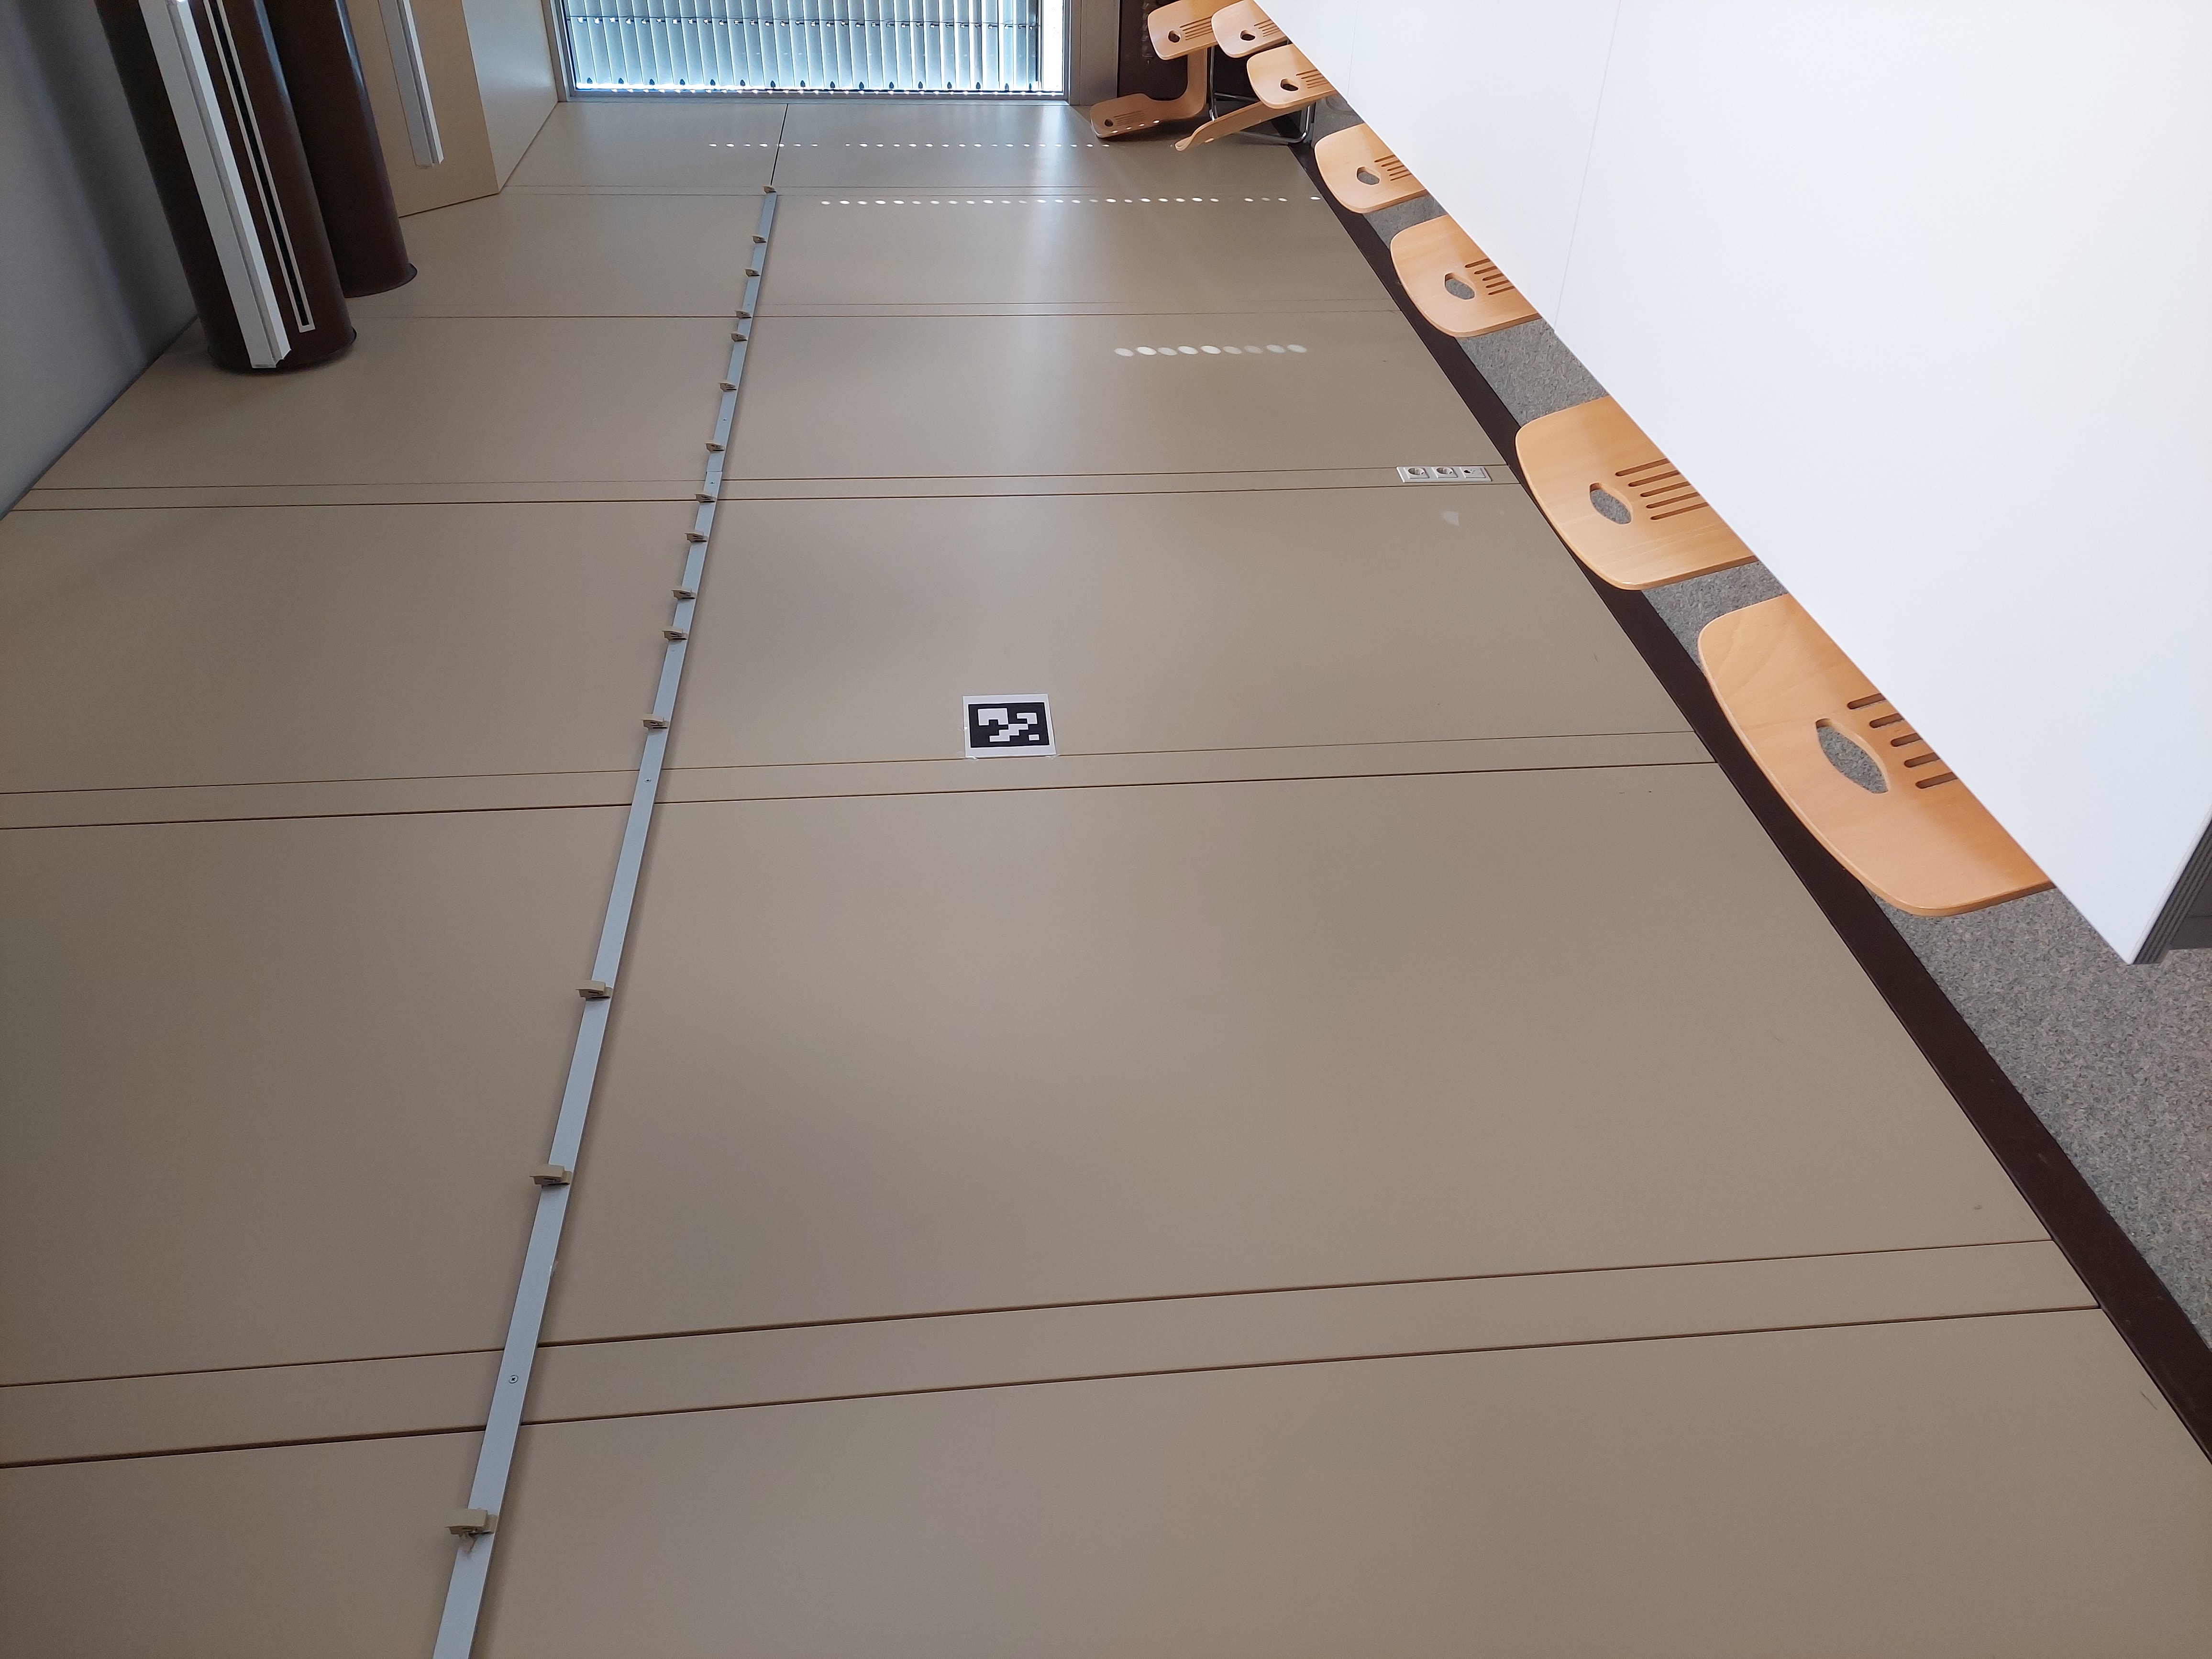
\includegraphics[width=0.9\columnwidth]{img/img_base_113340.jpg} % Beispielbild
    \caption{Fernaufame des Arucumarkers aus dem Vorgegbeenen Datensatz.}
    \label{fig:example-base}
\end{figure}
Für die Platzierung eines Objekts im Bild muss im ersten Schritt der Fluchtpunkt ermittelt werden, damit die korrekte Transformation auf das Objekt angewendet werden kann. Dazu wird der im Bild enthaltene Aruco-Marker genutzt. Hierfür verwenden wir die Funktion detectMarkers des aruco-Moduls von OpenCV. Dieses Modul liefert die Eckpunkte des Aruco-Markers zurück.
\\
Da der Aruco-Marker per Definition quadratisch ist, kann mithilfe der detektierten Eckpunkte der Fluchtpunkt berechnet werden. Dies wird durch die Funktion perspectiveTransform der OpenCV-Bibliothek ermöglicht. Nachdem die notwendige Transformation berechnet wurde, um das Poster im Raum zu platzieren, kann das Poster geladen und transformiert werden, ebenfalls mit der Funktion perspectiveTransform von OpenCV. Anschließend kann das transformierte Poster in das gewünschte Bild eingefügt werden.

\section{Ergebnisse}

Mithilfe des entwickelten Codes ist es nun möglich, durch eine Schleife auf alle gegebenen Bilder ein passendes transformiertes Poster zu platzieren. Um die Genauigkeit der Transformation ermitteln zu können, wird der jeweils ermittelte Fluchtpunkt in die Bilder eingezeichnet. Dies geschieht durch das Einfügen von Linien, die den Fluchtpunkt hervorheben.
\begin{figure}[h!]
    \centering
    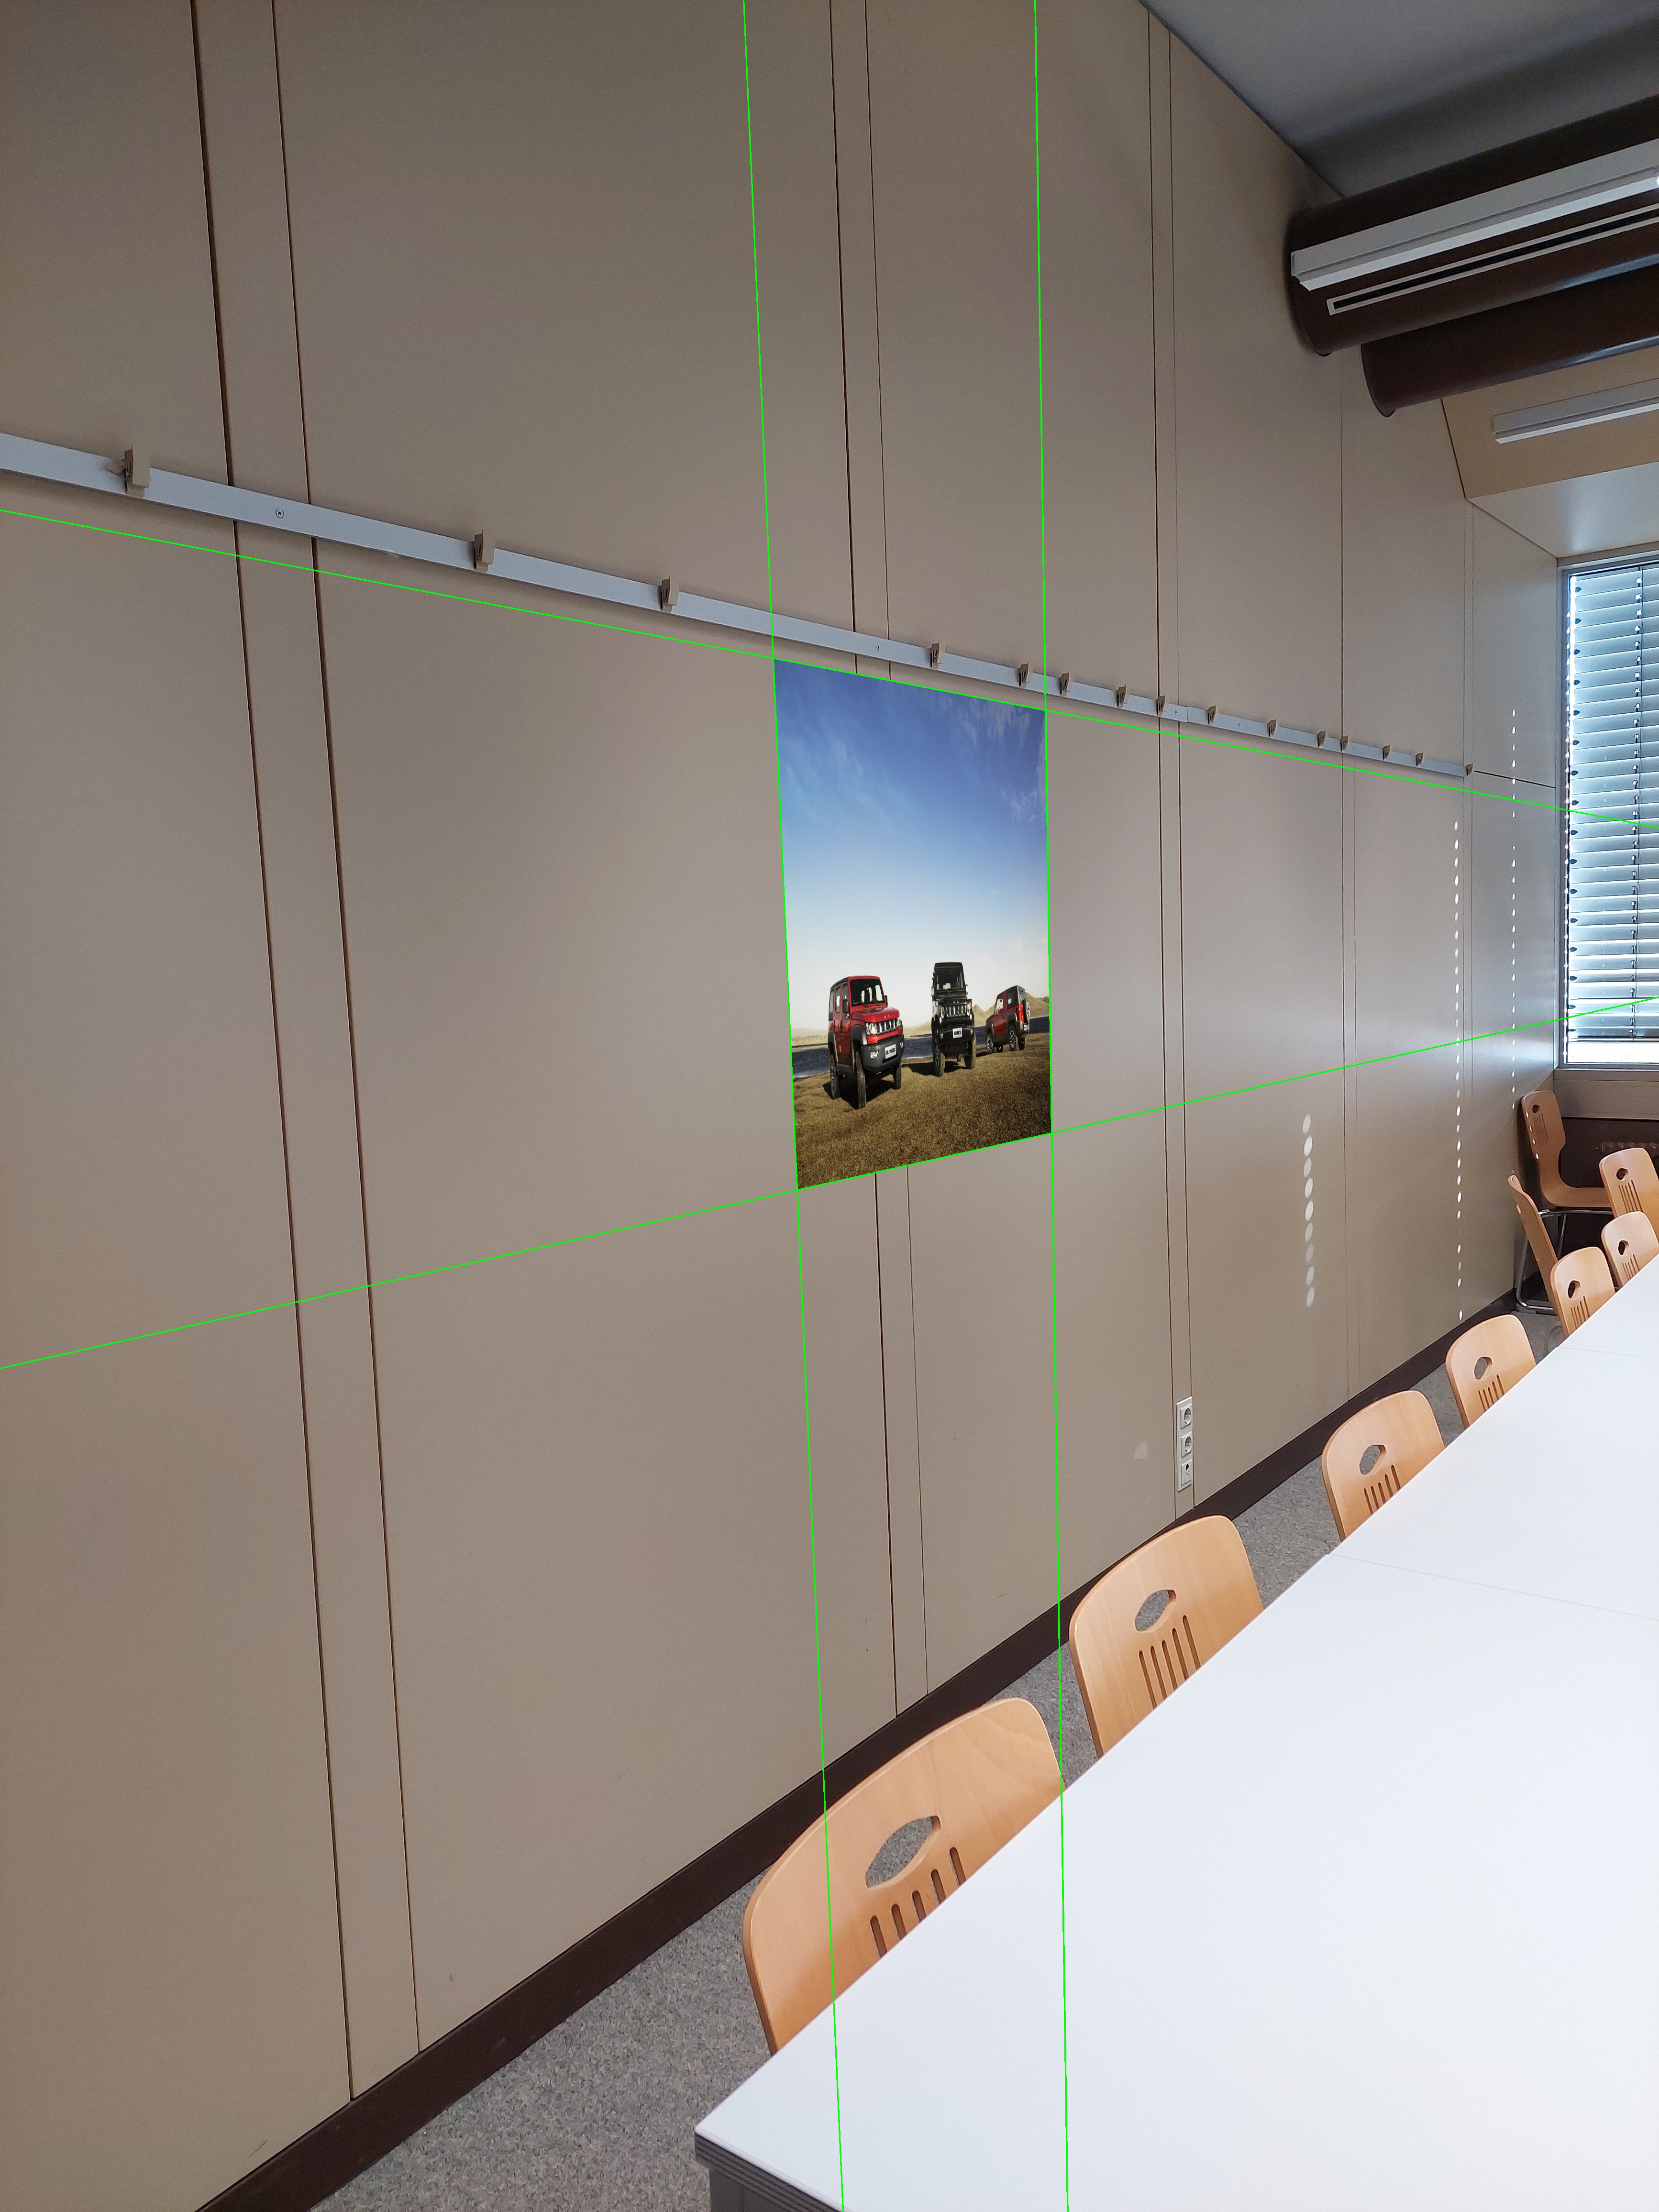
\includegraphics[width=0.9\columnwidth]{img/img_result_113340.jpg} % Beispielbild
    \caption{Fernaufame des Arucumarkers aus dem Vorgegbeenen Datensatz mit Poster.}
    \label{fig:example-result}
\end{figure}

Das transformierte Poster sowie die zugehörigen Fluchtpunktlinien in Grün sind in Abbildung \ref{fig:example-result} dargestellt. Eine schnelle Analyse der Ergebnisse ist in diesem Fall aufgrund der Beschaffenheit der Wand möglich. Der Vergleich der oberen horizontalen grünen Linie mit der Metallstange darüber zeigt, dass die angewendete Transformation korrekt auf die Verzerrung des Bildes angepasst wurde.
\\
Ähnliches gilt für die vertikalen Fluchtpunktlinien und die Lücken zwischen den Wandpanelen. Daraus lässt sich ableiten, dass der entwickelte Code grundsätzlich auf Bilddateien mit Aruco-Markern anwendbar ist.
\\
Bei der Analyse weiterer Bilder zeigt sich jedoch, dass die Erkennung des Aruco-Markers nicht in jeder Perspektive zuverlässig funktioniert. Ein Beispiel hierfür ist in Abbildung \ref{fig:bad-example-result} zu sehen. Beim Vergleich der horizontalen Fluchtpunktlinien mit der Metallstange wird sichtbar, dass die Fluchtpunktlinien mit zunehmender Entfernung immer weiter von der Stange abweichen und schließlich in einem Punkt enden.\begin{figure}[h!]
    \centering
    \includegraphics[width=0.9\columnwidth]{img/img_result_bad_113437.jpg} % Beispielbild
    \caption{Beispiel für eine Perspektive bei welcher der Fluchtpunkt schlecht erkannt wurde.}
    \label{fig:bad-example-result}
\end{figure}

section{Fazit und Ausblick}

Im Rahmen dieses Projekts wurde eine Software zur Platzierung von Postern in einem Bild entwickelt. Dafür wurden hauptsächlich der Aruco-Marker und die Bibliothek OpenCV verwendet.
\\
Die Ergebnisse der Posterplatzierung sind grundsätzlich solide und positionieren das Poster in der richtigen Größe im Raum. Die Abweichung zwischen der berechneten und der tatsächlichen Verzerrung ist in den analysierten Bildern so geringfügig, dass die Fehler nicht störend wirken.
\\
Eine Verbesserung der Fluchtpunktberechnung war im zeitlichen Umfang dieser Arbeit nicht möglich und könnte im Rahmen einer umfangreicheren wissenschaftlichen Untersuchung weiter optimiert werden.

%\begin{thebibliography}{99}
%\bibitem{ref1} Autor, Titel, Quelle, Jahr.
%\bibitem{ref2} Autor, Titel, Quelle, Jahr.
%\end{thebibliography}

%\end{document}
\begin{thebibliography}{9}
    \bibitem{aruco}
    \todo{Quelle nochmal prüfen. Prof ist wirklich streng!}
    S. Garrido-Jurado, R. Muñoz-Salinas, F. J. Madrid-Cuevas, M. J. Marín-Jiménez. 
    \textit{Automatic generation and detection of highly reliable fiducial markers under occlusion}. Pattern Recognition, vol. 11, no 6, 2021.

\end{thebibliography}
\todo{Hinzufügen der anderen Bilder}

\end{document}